\subsection{ソフトウェアアーキテクチャの基礎}

\subsubsection{「アーキテクチャ」という語の意味}
ソフトウェア工学では、「アーキテクチャ」という語が少なくとも三つの意味で使われる。

第一に、アーキテクチャは\term{分野}{Discipline}を指す。これは、ソフトウェア集約システムを構成するための考え方、原則、過程、方法を扱う知識領域である。建築における建築学が、建物をどう構成するかを扱うのと同じように、ソフトウェアアーキテクチャは、ソフトウェア集約システムをどう構成するかを扱う。

第二に、アーキテクチャは\term{活動}{Activity}を指す。アーキテクチャを作る活動は、しばしば「アーキテクチャ設計」または「アーキテクティング」と呼ばれる。ソフトウェア設計は、一般にアーキテクチャ設計、高水準設計、詳細設計に分けられる。この章は、その中でも根本的な構造や重要な意思決定に関わる部分を扱う。

第三に、アーキテクチャは\term{成果}{Result}を指す。つまり、あるシステムについて、主要な構成要素、関係、原則、設計判断がどのようになっているかという結果である。この成果は、アーキテクチャ記述として表される。

かつての定義では、アーキテクチャは「システムまたは構成要素の組織構造」と理解されることが多かった。しかし、現代の考え方では、単なる構造だけでは足りない。ソフトウェアには、コード構造だけでなく、実行時構造、配置構造、情報構造、開発組織との対応、運用構造など、複数の構造がある。また、アーキテクチャは環境の中のシステムとして考える必要がある。

\begin{definitionbox}
ソフトウェアアーキテクチャとは、システムの環境における根本的な概念または性質であり、構成要素、構成要素間の関係、設計と進化の原則として表れるものである。
\end{definitionbox}

この定義の要点は二つである。第一に、アーキテクチャはすべての詳細を含むものではなく、根本的なものを扱う。第二に、アーキテクチャはシステムの外側も見る。利用者、組織、外部システム、ハードウェア、法律、規制、運用環境などとの関係が重要である。

\par\smallskip
\begin{center}
\centering
\IfFileExists{assets/generated_figures/ch02/fig-ch02-02.png}{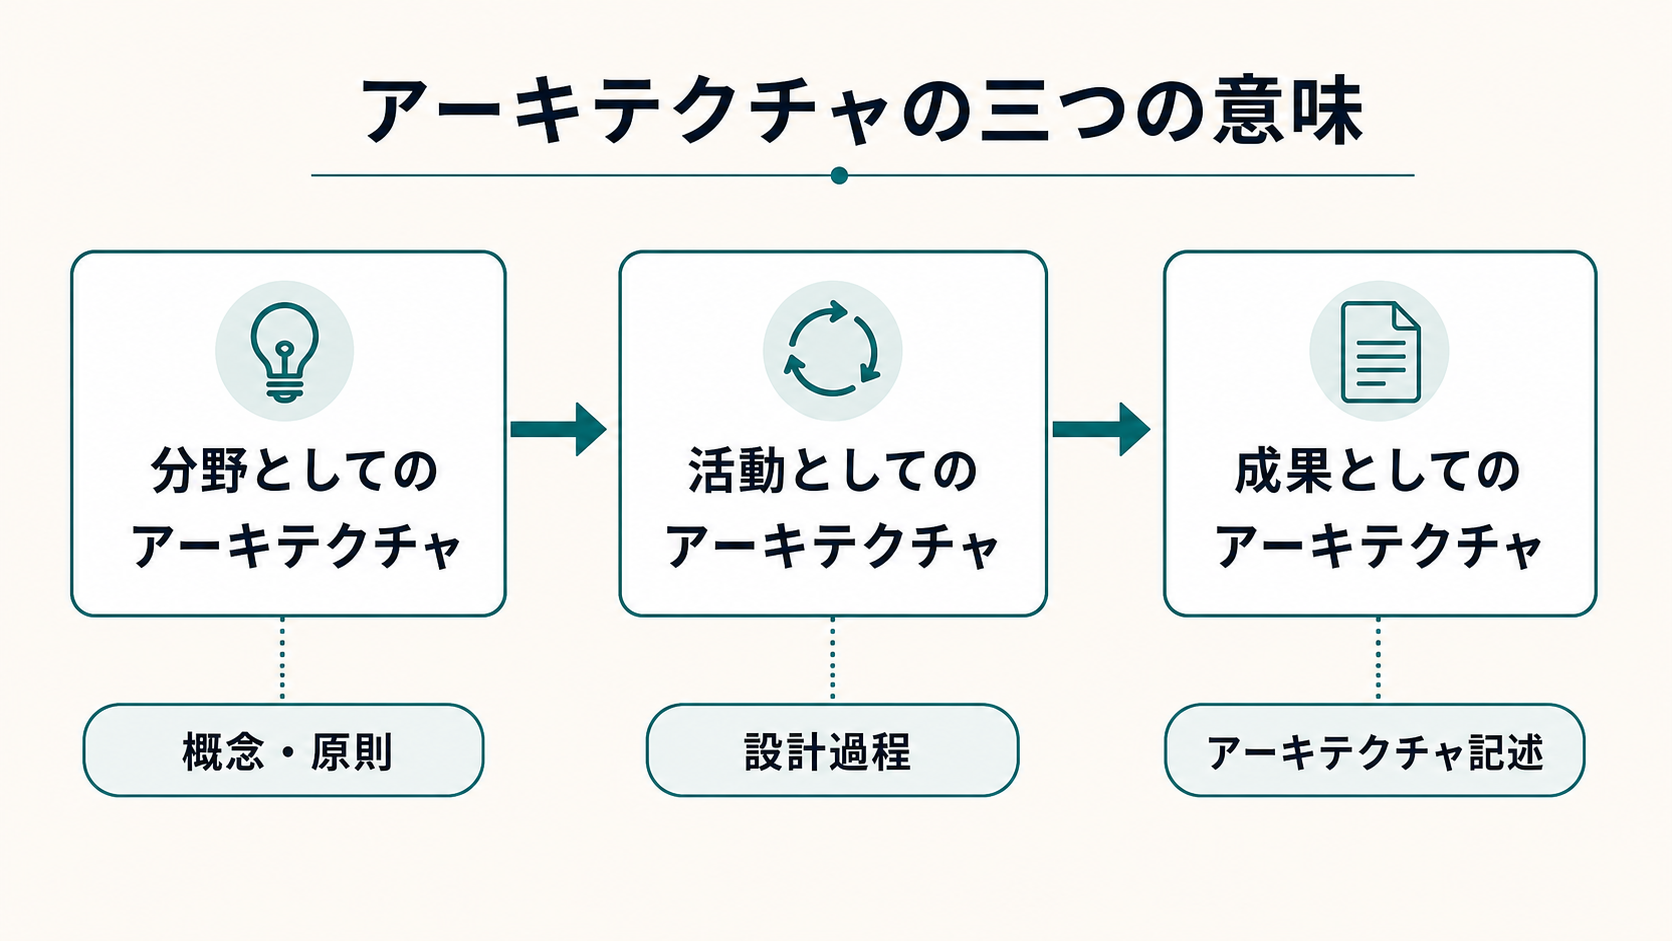
\includegraphics[width=0.96\linewidth]{assets/generated_figures/ch02/fig-ch02-02.png}}{\fbox{\parbox[c][48mm][c]{0.9\linewidth}{\centering 画像生成待ち\\アーキテクチャの三つの意味}}}
\par\smallskip
\refstepcounter{figure}\label{fig:ch02-02}図 \thefigure: アーキテクチャの三つの意味
\end{center}
図 \thefigure は、アーキテクチャの三つの意味を視覚的に整理したものである。
\par\smallskip

\subsubsection{利害関係者と関心事}
ソフトウェアシステムには、多くの利害関係者がいる。顧客は、いつ完成するか、いくらかかるか、投資に見合う価値があるかを気にする。利用者は、何ができるか、使いやすいか、作業を妨げないかを気にする。開発者は、構成要素の責任、インタフェース、依存関係、実装しやすさを気にする。運用担当は、配置、監視、障害対応、復旧、性能を気にする。保守担当は、変更しやすさ、影響範囲のわかりやすさ、技術的負債を気にする。

このような「気にする論点」を関心事という。アーキテクチャの重要な役割は、利害関係者ごとの関心事を整理し、それぞれに答えられる表現を用意することである。

\begin{statementbox}{関心事の分離}
複雑なシステムを一度にすべて理解しようとすると、論点が混ざる。関心事の分離とは、性能、安全性、セキュリティ、使いやすさ、保守性などを、必要に応じて分けて考える方法である。分けることは、他の関心事を無視することではなく、順序立てて考えるための技法である。
\end{statementbox}

関心事は、機能的なもの、非機能的なもの、制約の形を取るものに分けられる。さらに、技術、事業、運用、組織、政治、経済、法令、規制、環境、社会的影響など、非常に広い範囲にまたがる。近年は、気候変動への意識の高まりにより、エネルギー効率や持続可能性もアーキテクチャ上の関心事になっている。

\par\smallskip\noindent\refstepcounter{table}\label{tab:ch02-02}表 \thetable: 利害関係者と関心事における利害関係者・典型的な関心事\par\smallskip
表 \thetable は、利害関係者と関心事における利害関係者・典型的な関心事を比較・確認しやすい形で整理したものである。\par\smallskip
\begin{longtable}{P{0.25\linewidth}P{0.67\linewidth}}
\toprule
利害関係者 & 典型的な関心事 \\
\midrule
顧客・発注者 & 費用、納期、事業価値、契約適合性、長期的な運用費である。 \\
利用者 & 機能、使いやすさ、応答時間、信頼性、利用体験である。 \\
開発者 & 構成要素の責任、インタフェース、依存関係、実装容易性、テスト容易性である。 \\
運用担当 & 配置、監視、可用性、障害復旧、容量、セキュリティ運用である。 \\
保守担当 & 変更容易性、理解しやすさ、技術的負債、互換性である。 \\
監査・認証担当 & 法令・規格への適合、証拠、説明可能性、安全性、セキュリティである。 \\
\bottomrule
\end{longtable}

\par\smallskip
\begin{center}
\centering
\IfFileExists{assets/generated_figures/ch02/fig-ch02-03.png}{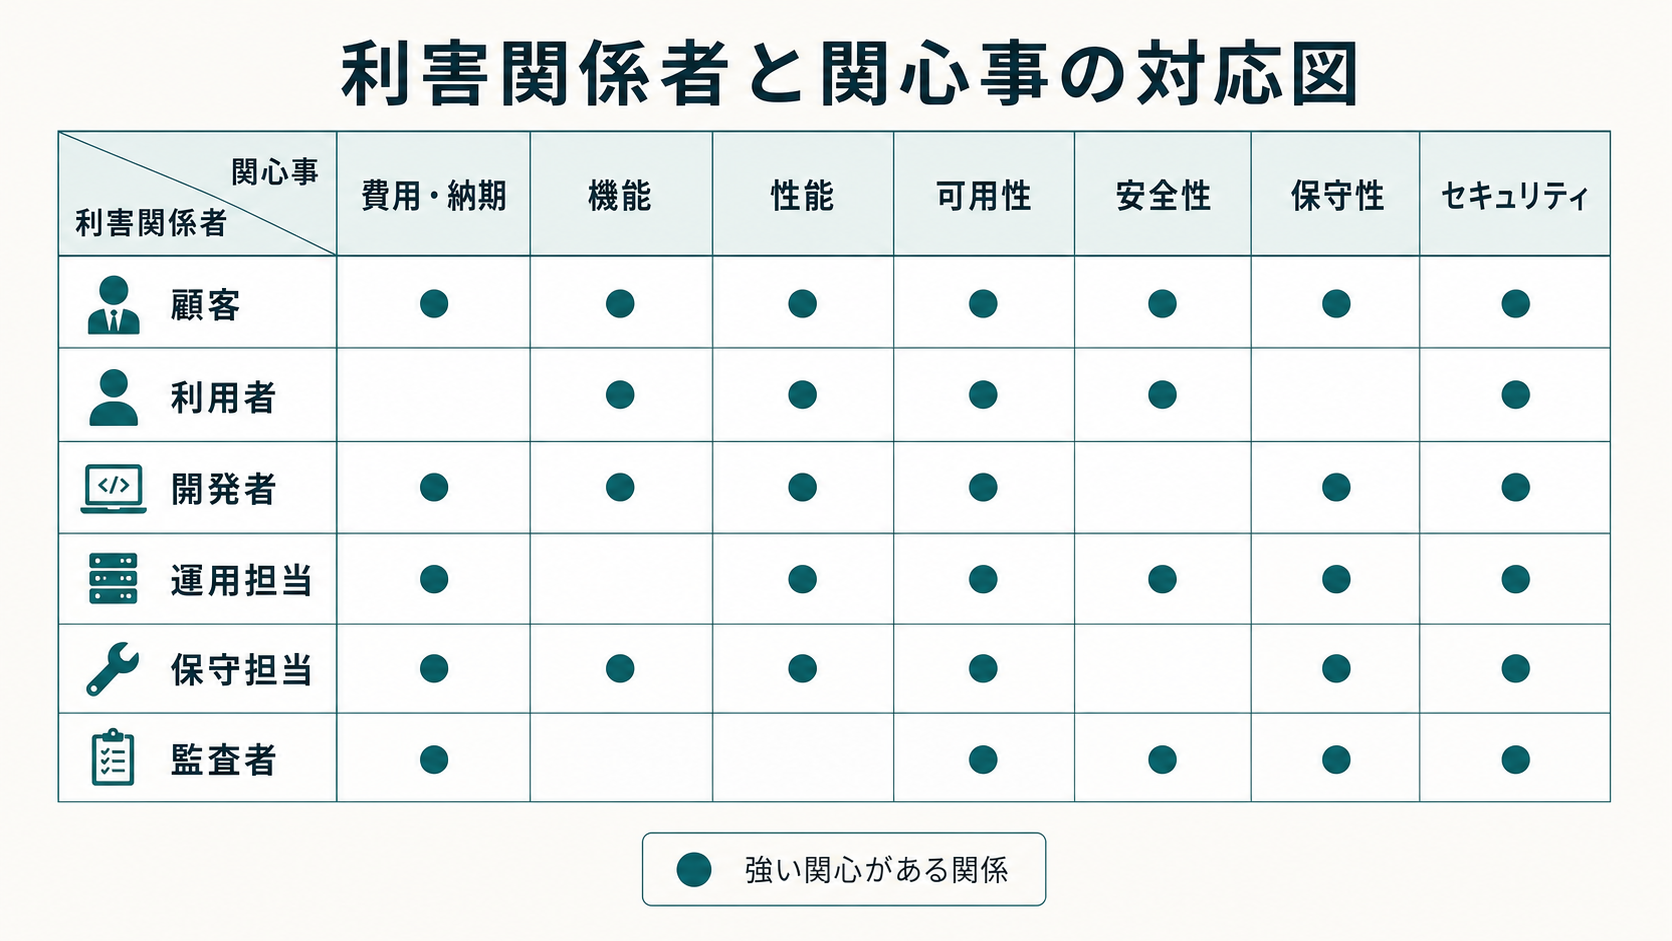
\includegraphics[width=0.96\linewidth]{assets/generated_figures/ch02/fig-ch02-03.png}}{\fbox{\parbox[c][48mm][c]{0.9\linewidth}{\centering 画像生成待ち\\利害関係者と関心事の対応図}}}
\par\smallskip
\refstepcounter{figure}\label{fig:ch02-03}図 \thefigure: 利害関係者と関心事の対応図
\end{center}
図 \thefigure は、利害関係者と関心事の対応図を視覚的に整理したものである。
\par\smallskip

\subsubsection{アーキテクチャの用途}
アーキテクチャの第一の用途は、システムに関わる人々が共有理解を持つことである。共有理解がなければ、設計者、開発者、テスト担当、運用担当が異なる前提で作業し、結果として整合しないシステムになりやすい。

第二の用途は、設計と構築の指針を与えることである。アーキテクチャは、どの構成要素が存在するか、どの構成要素がどの責任を持つか、どのように通信するか、どの品質特性をどの方法で満たすかを示す。これにより、実装前に代替案を比較し、リスクを見つけられる。

第三の用途は、既存システムの理解である。保守、拡張、移行、改善を行うとき、既存システムのアーキテクチャを理解することが重要である。これは、逆方向の設計理解、すなわちリバースアーキテクティングに近い活動である。

また、アーキテクチャは組織構造とも関係する。コンウェイの法則は、システムの構造が、それを設計する組織のコミュニケーション構造を反映しやすいことを指摘する。組織とアーキテクチャの対応は、うまく使えば分担と責任を明確にする力になるが、悪く働くと不要な分断や複雑な依存関係を生む。

\begin{statementbox}{実務での見方}
アーキテクチャは、計画、見積り、分担、再利用、製品系列化にも使われる。単一システムの内部構造だけでなく、複数製品に共通する土台を作るためにも重要である。
\end{statementbox}
